\documentclass[12pt, a4paper]{article}

\usepackage[utf8]{inputenc}
\usepackage[T1]{fontenc}
\usepackage[pdftex]{graphicx}
\usepackage{booktabs}
\usepackage{amsmath}
\usepackage{amssymb}
\usepackage[left=2.5cm,right=2.5cm,top=3cm,bottom=3.5cm]{geometry}
\usepackage{indentfirst}
\usepackage[activate={true,nocompatibility},final,tracking=true,kerning=true,spacing=true,factor=1100,stretch=10,shrink=10]{microtype}
\usepackage{float}
\usepackage[small, it]{caption}

\renewcommand{\figurename}{Slika}

\microtypecontext{spacing=nonfrench}

\allowdisplaybreaks

\title{Neizrazito, evolucijsko i neuroračunarstvo:\\
  Izvješće uz 7. laboratorijsku vježbu -- \\Klasifikacija umjetnom neuronskom mrežom treniranom genetskim algoritmom}
\author{Lovre Mrčela}

\date{13. siječnja 2017.}

\begin{document}

\maketitle

\paragraph{Zadatak 1.}
Razmotrite jedan neuron koji ima samo jedan ulaz.
Njegov izlaz tada će biti određen izrazom:

$$ y= \dfrac{1}{1 + \dfrac{|x - w|}{|s|}}$$
Pretpostavite da je u neuron pohranjena vrijednost $w=2$. Nacrtajte \textit{na istom grafu} ovisnost $y(x; w=2)$ za tri slučaja: za $s=1$, za $s=0.25$, te za $s=4$ (svaku različitom bojom ili stilom linije). Za raspon apscise uzmite interval $[-8, 10]$. Razumijete li sada kako $s$ utječe na izlaz neurona $y$? Kako će izgledati izlaz neurona koji ima dva ulaza i što se tada kontrolira parametrima $s_1$ i $s_2$?\\

\noindent\textsc{Rješenje:}
\begin{figure}[p]
  \centering
  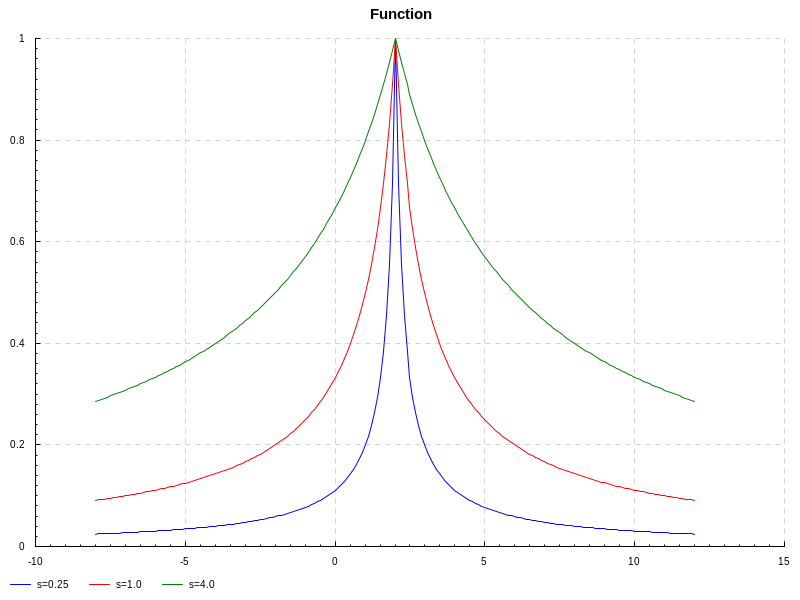
\includegraphics[width=0.8\linewidth]{function.png}
  \caption{Izgled aktivacijske funkcije neurona iz zadatka uz tri različite vrijednosti parametra $s$.}
  \label{fig:function}
\end{figure}
Graf je prikazan na slici \ref{fig:function}.
Slika je generirana u programskom kodu.
Veličina $s$ utječe na širinu područja koje ``prolazi'' kroz nju.
U slučaju dvaju ulaza, svaki parametar regulira širinu svoga područja koje ``propušta''.

\paragraph{Zadatak 2.}
Iskoristite neki gotov program (ili napišite vlastiti program, što god Vam je lakše) kako biste dobili 2D prikaz podataka koje ste dobili za učenje (\texttt{zad-7-dataset.txt}).
Pri tome uzorke različitih razreda prikažite ili različitim simbolom (npr. kvadratić, trokutić, kružić) ili različitom bojom.
Ovu sliku spremite kao dio Vaše dokumentacije.
Ako ste koristili gotov program, navedite naziv programa.
Proučite dobiveni prikaz. Postoji li kakav uzorak u tim podatcima?
Jesu li razredi međusobno linearno odvojivi?\\

\noindent\textsc{Rješenje:}
\begin{figure}[p]
  \centering
  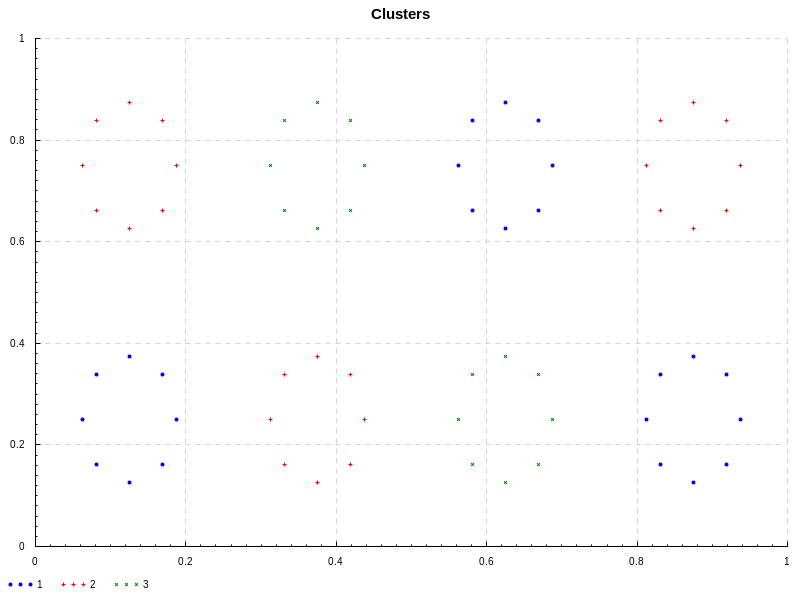
\includegraphics[width=0.8\linewidth]{clusters.png}
  \caption{Izgled primjera za učenje u prostoru značajki.}
  \label{fig:clusters}
\end{figure}
Graf je prikazan na slici \ref{fig:clusters}.
Slika je generirana u programskom kodu.
Razredi nisu linearno odvojivi.
Međutim, razredi su kompaktno smješteni unutar 8 područja, što ostavlja mogućnost da se svi primjer ispravno klasificiraju upotrebom neuronske mreže koja ima barem 8 čvorova u sloju tipa 1.

\paragraph{Zadatak 3.}
Kada biste morali ručno odrediti vrijednosti svih parametara upravo zadane neuronske mreže ($2\times8\times3$), na koje biste ih vrijednosti postavili i zašto?
Čime biste se vodili prilikom određivanja parametara neurona izlaznog sloja?
Nacrtajte tu neuronsku mrežu i na njoj prikažite vrijednosti svih parametara.\\

\noindent\textsc{Rješenje:}
Parametri neuronske mreže bili bi postavljeni na način da $w$-ovi u sloju tipa 1 odgovaraju centrima 8 područja u koja su smješteni pojedini razredi, $s$-ovi odgovaraju širini područja, te $w$-ovi u sloju tipa 2 budu 1 za ona područja koja pripadaju tom razredu, inače 0. Parametri bi bili sljedeći:
\begin{itemize}
  \item 1. sloj: \textit{nema parametara},
  \item 2. sloj (tip 1):
  \begin{itemize}
    \item 1. čvor: $w_1=\frac{1}{8}, s_1=\frac{1}{4}, w_2=\frac{1}{4}, s_2=\frac{1}{2}$,
    \item 2. čvor: $w_1=\frac{3}{8}, s_1=\frac{1}{4}, w_2=\frac{1}{4}, s_2=\frac{1}{2}$,
    \item 3. čvor: $w_1=\frac{5}{8}, s_1=\frac{1}{4}, w_2=\frac{1}{4}, s_2=\frac{1}{2}$,
    \item 4. čvor: $w_1=\frac{7}{8}, s_1=\frac{1}{4}, w_2=\frac{1}{4}, s_2=\frac{1}{2}$,
    \item 5. čvor: $w_1=\frac{1}{8}, s_1=\frac{1}{4}, w_2=\frac{3}{4}, s_2=\frac{1}{2}$,
    \item 6. čvor: $w_1=\frac{3}{8}, s_1=\frac{1}{4}, w_2=\frac{3}{4}, s_2=\frac{1}{2}$,
    \item 7. čvor: $w_1=\frac{5}{8}, s_1=\frac{1}{4}, w_2=\frac{3}{4}, s_2=\frac{1}{2}$,
    \item 8. čvor: $w_1=\frac{7}{8}, s_1=\frac{1}{4}, w_2=\frac{3}{4}, s_2=\frac{1}{2}$,
  \end{itemize}
  \item 3. sloj (tip 2):
  \begin{itemize}
    \item 1. čvor: $w_1=0, w_2=0, w_3=1, w_4=0, w_5=1, w_6=0, w_7=0, w_8=1, b=0$,
    \item 2. čvor: $w_1=1, w_2=0, w_3=0, w_4=1, w_5=0, w_6=1, w_7=0, w_8=0, b=0$,
    \item 3. čvor: $w_1=0, w_2=1, w_3=0, w_4=0, w_5=0, w_6=0, w_7=1, w_8=0, b=0$.
  \end{itemize}
\end{itemize}

\paragraph{Zadatak 4.}
Naučite optimalne parametre mreže arhitekture $2\times8\times3$.
Nacrtajte novu sliku na kojoj se vide svi ulazni uzorci s indikacijom razreda te uzorci koje je GA naučio za svaki neuron tipa 1.
Prokomentirajte gdje se nalaze naučeni uzorci i je li to u skladu s očekivanjem.
Kakve je vrijednosti parametara $s_i$ naučio GA?
Jesu li iste za $x$ i $y$ komponentu ili su različite?
Objasnite!
Nacrtajte novu sliku na kojoj se vide svi neuroni neuronske mreže, pozicije koje su naučene u neuronima tipa 1 te vrijednosti težina za neurone tipa 2.
Uočavate li kakvu pravilnost u tim težinama?
Možete li je objasniti?\\

\noindent\textsc{Rješenje:}
Izgled naučenih centroida prikazan je na slici \ref{fig:trained}.
Naučeni centroidi daleko odskaču od pretpostavljenih iz prethodnog zadatka.
Naučene težine u trećem sloju su:
\begin{itemize}
  \item 1. čvor: $w_1=237.70, w_2=289.31, w_3=-235.88, w_4=-158.85, w_5=-128.27, w_6=-171.67, w_7=226.45, w_8=154.64, b=15.68$,
  \item 2. čvor: $w_1=-102.41, w_2=-125.71, w_3=127.71, w_4=66.13, w_5=130.72, w_6=124.49, w_7=-91.07, w_8=-133.29, b=-44.33$,
  \item 3. čvor: $w_1=-227.57, w_2=237.62, w_3=-55.31, w_4=-120.01, w_5=-1048.72, w_6=-122.92, w_7=-461.85, w_8=127.66, b=350.57$.
\end{itemize}
Možemo primijetiti kako su i ove težine ``eksplodirale''.
Unatoč tome, klasifikacijska pogreška je ispod $10^{-7}$.

\begin{figure}[p]
  \centering
  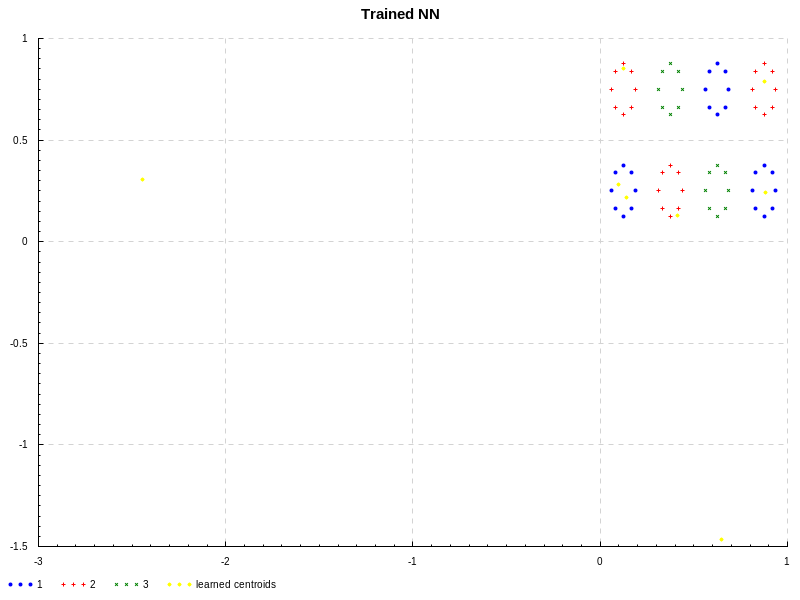
\includegraphics[width=0.8\linewidth]{trained.png}
  \caption{Izgled naučenih centroida iz sloja 1 za mrežu $2\times8\times3$.}
  \label{fig:trained}
\end{figure}

\paragraph{Zadatak 5.}
Naučite optimalne parametre mreže $2\times8\times4\times3$.
Je li postupak učenja trajao dulje ili kraće u odnosu na prethodnu arhitekturu?
Možete li objasniti zašto?
Pogledajte naučene parmetre u neuronima tipa 1 za ovaj slučaj.
Možete li ih objasniti?\\

\noindent\textsc{Rješenje:}
Trajanje treniranja do ukupne srednje pogreške koja je ispod $10^{-7}$ je znatno kraće u ovom slučaju (4315 iteracija) nego u prethodnom (29071 iteracija).
Izgled naučenih centroida prikazan je na slici \ref{fig:trained2}.
I u ovom slučaju centroidi su razbacani po čitavom prostoru značajki.

\begin{figure}[p]
  \centering
  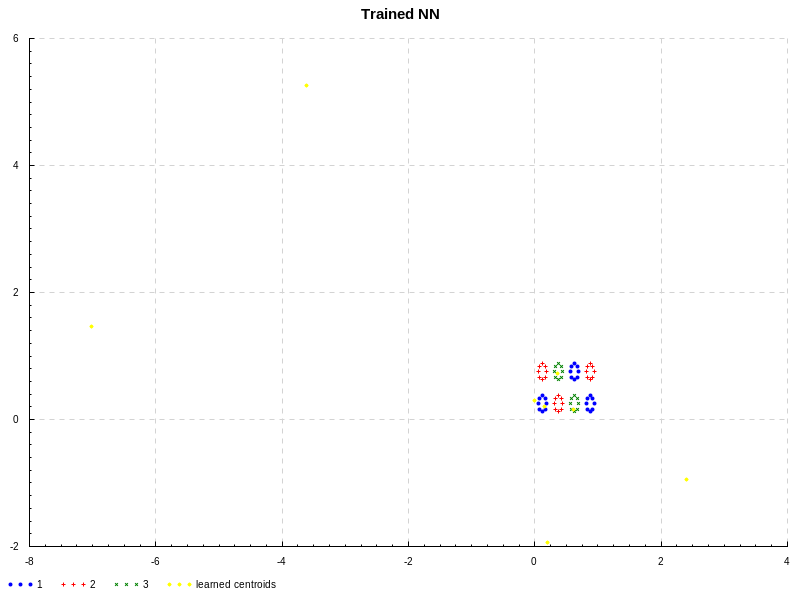
\includegraphics[width=0.8\linewidth]{trained2.png}
  \caption{Izgled naučenih centroida iz sloja 1 za mrežu $2\times8\times4\times3$.}
  \label{fig:trained2}
\end{figure}

\paragraph{Zadatak 6.}
Možete li dobiti ispravnu klasifikaciju svih uzoraka u arhitekturi koja ima $N_1 < 8$?
Provjerite to na arhitekturi $2 \times 6 \times 4 \times 3$.
Na kraju (uspješnog ili neuspješnog) postupka učenja pogledajte za najbolje rješenje parametre u neuronima tipa 1 za ovaj slučaj.
Što smo izgubili u odnosu na mrežu iz zadatka 4?

\noindent\textsc{Rješenje:}
Trajanje treniranja u ovom slučaju je bilo 4258 iteracija.
Izgled naučenih centroida prikazan je na slici \ref{fig:trained3}.
U usporedbi sa zadatkom 5 centroidi su ``razbacani'' na užem području, a u usporedbi sa zadatkom 4 na širem.

\begin{figure}[p]
  \centering
  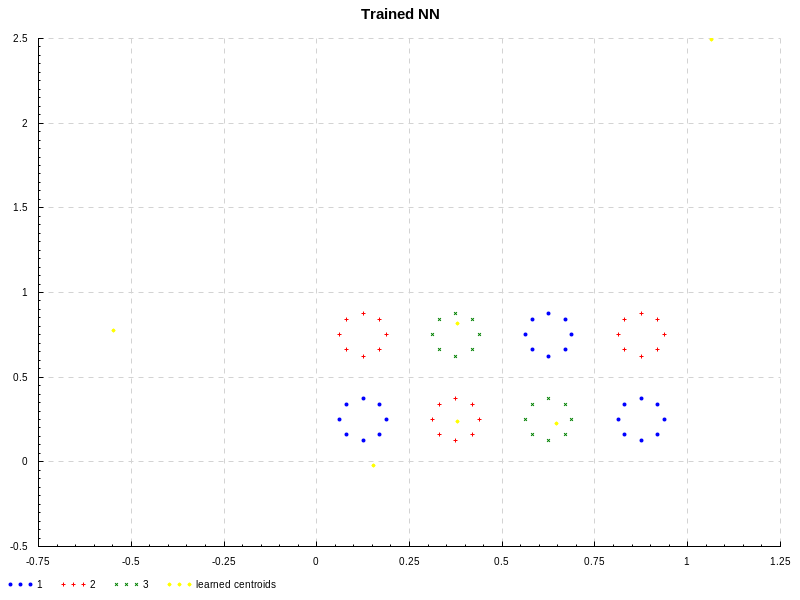
\includegraphics[width=0.8\linewidth]{trained3.png}
  \caption{Izgled naučenih centroida iz sloja 1 za mrežu $2\times6\times4\times3$.}
  \label{fig:trained3}
\end{figure}

\end{document}
